% Options for packages loaded elsewhere
\PassOptionsToPackage{unicode}{hyperref}
\PassOptionsToPackage{hyphens}{url}
%
\documentclass[
]{ctexart}
\usepackage{amsmath,amssymb}
\usepackage{lmodern}
\usepackage{iftex}
\ifPDFTeX
  \usepackage[T1]{fontenc}
  \usepackage[utf8]{inputenc}
  \usepackage{textcomp} % provide euro and other symbols
\else % if luatex or xetex
  \usepackage{unicode-math}
  \defaultfontfeatures{Scale=MatchLowercase}
  \defaultfontfeatures[\rmfamily]{Ligatures=TeX,Scale=1}
\fi
% Use upquote if available, for straight quotes in verbatim environments
\IfFileExists{upquote.sty}{\usepackage{upquote}}{}
\IfFileExists{microtype.sty}{% use microtype if available
  \usepackage[]{microtype}
  \UseMicrotypeSet[protrusion]{basicmath} % disable protrusion for tt fonts
}{}
\makeatletter
\@ifundefined{KOMAClassName}{% if non-KOMA class
  \IfFileExists{parskip.sty}{%
    \usepackage{parskip}
  }{% else
    \setlength{\parindent}{0pt}
    \setlength{\parskip}{6pt plus 2pt minus 1pt}}
}{% if KOMA class
  \KOMAoptions{parskip=half}}
\makeatother
\usepackage{xcolor}
\usepackage{graphicx}
\makeatletter
\def\maxwidth{\ifdim\Gin@nat@width>\linewidth\linewidth\else\Gin@nat@width\fi}
\def\maxheight{\ifdim\Gin@nat@height>\textheight\textheight\else\Gin@nat@height\fi}
\makeatother
% Scale images if necessary, so that they will not overflow the page
% margins by default, and it is still possible to overwrite the defaults
% using explicit options in \includegraphics[width, height, ...]{}
\setkeys{Gin}{width=\maxwidth,height=\maxheight,keepaspectratio}
% Set default figure placement to htbp
\makeatletter
\def\fps@figure{htbp}
\makeatother
\setlength{\emergencystretch}{3em} % prevent overfull lines
\providecommand{\tightlist}{%
  \setlength{\itemsep}{0pt}\setlength{\parskip}{0pt}}
\setcounter{secnumdepth}{5}
\ifLuaTeX
  \usepackage{selnolig}  % disable illegal ligatures
\fi
\IfFileExists{bookmark.sty}{\usepackage{bookmark}}{\usepackage{hyperref}}
\IfFileExists{xurl.sty}{\usepackage{xurl}}{} % add URL line breaks if available
\urlstyle{same} % disable monospaced font for URLs
\hypersetup{
  pdftitle={Biostatistical Note},
  pdfauthor={Haoxi Ma},
  pdfkeywords={中文, R Markdown},
  hidelinks,
  pdfcreator={LaTeX via pandoc}}

\title{Biostatistical Note}
\author{Haoxi Ma}
\date{2021-10-10}

\begin{document}
\maketitle

\begin{center}\rule{0.5\linewidth}{0.5pt}\end{center}

\hypertarget{clinical-trials}{%
\subsubsection{\texorpdfstring{\textbf{Clinical
Trials}}{Clinical Trials}}\label{clinical-trials}}

\hypertarget{phases}{%
\paragraph{Phases}\label{phases}}

Clinical trials are systematically designed, set of activities that are
done to verify the safety and efficacy of an investigational new drug
(IND).

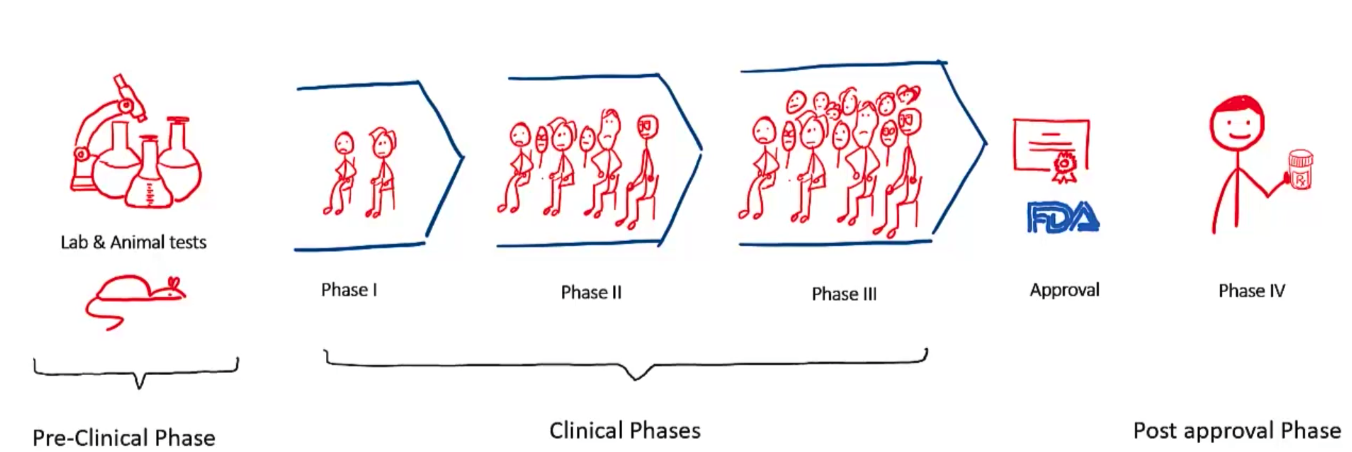
\includegraphics{/post/2021-10-10-biostatistical-note_files/1.jpg}

\begin{itemize}
\item
  \textbf{Phase I trial} tests an experimental treatment on a small
  group of often healthy people (20 to 80) to judge its safety and side
  effects and to find the correct drug dosage.
\item
  \textbf{Phase II trial} uses more people (100 to 300). While the
  emphasis in Phase I is on safety, the emphasis in Phase II is on
  effectiveness. This phase aims to obtain preliminary data on whether
  the drug works in people who have a certain disease or condition.
  These trials also continue to study safety, including short-term side
  effects. This phase can last several years.
\item
  \textbf{Phase III trial} gathers more information about safety and
  effectiveness, studying different populations and different dosages,
  using the drug in combination with other drugs. The number of subjects
  usually ranges from several hundred to about 3,000 people. If the FDA
  agrees that the trial results are positive, it will approve the
  experimental drug or device.
\item
  \textbf{Phase IV trial} for drugs or devices takes place after the FDA
  approves their use. A device or drug's effectiveness and safety are
  monitored in large, diverse populations. Sometimes, the side effects
  of a drug may not become clear until more people have taken it over a
  longer period of time.
\end{itemize}

\hypertarget{regulations}{%
\paragraph{Regulations}\label{regulations}}

\textbf{Clinical Data Interchange Standards Consortium (CDISC)} A
non-profit group that defines clinical data standards for the
pharmaceutical industry. CDISC has developed numerous data models that
you should familiarize yourself with. Two key sets of standards that
affect the majority of clinical trail programmers are the Study Data
Tabulation Model (SDTM) used for submitting data tabulations and the
Analysis Data Set Model (ADaM) used for submitting analysis datasets.
While these two sets of standards overlap in many areas, both have many
distinct components that can affect how data is stored.

Some sponsors might label gender as 0 or 1, while some might use
``Female'' or ``Male'', so SDTM gives a standard that gender should be
formatted as F or M when putting into public. ADaM datasets include
variables taken directly from SDTM as well as additional derived
variables.

Besides, SDTM and ADaM, Clinical Data Acquisition Standards
Harmonization (CDASH) is also widely used, which provides guidance to
develop the CRF for the domains that are commonly used for the majority
of the clinical trials across the therapeutic areas.

\textbf{Classify Clinical Trial Data based on SDTM} The data are broadly
classified as efficacy data and safety data. CDISC have categorized data
into interventions class, events class, finding class, and other
special-purpose ``domains'' such as demographics.

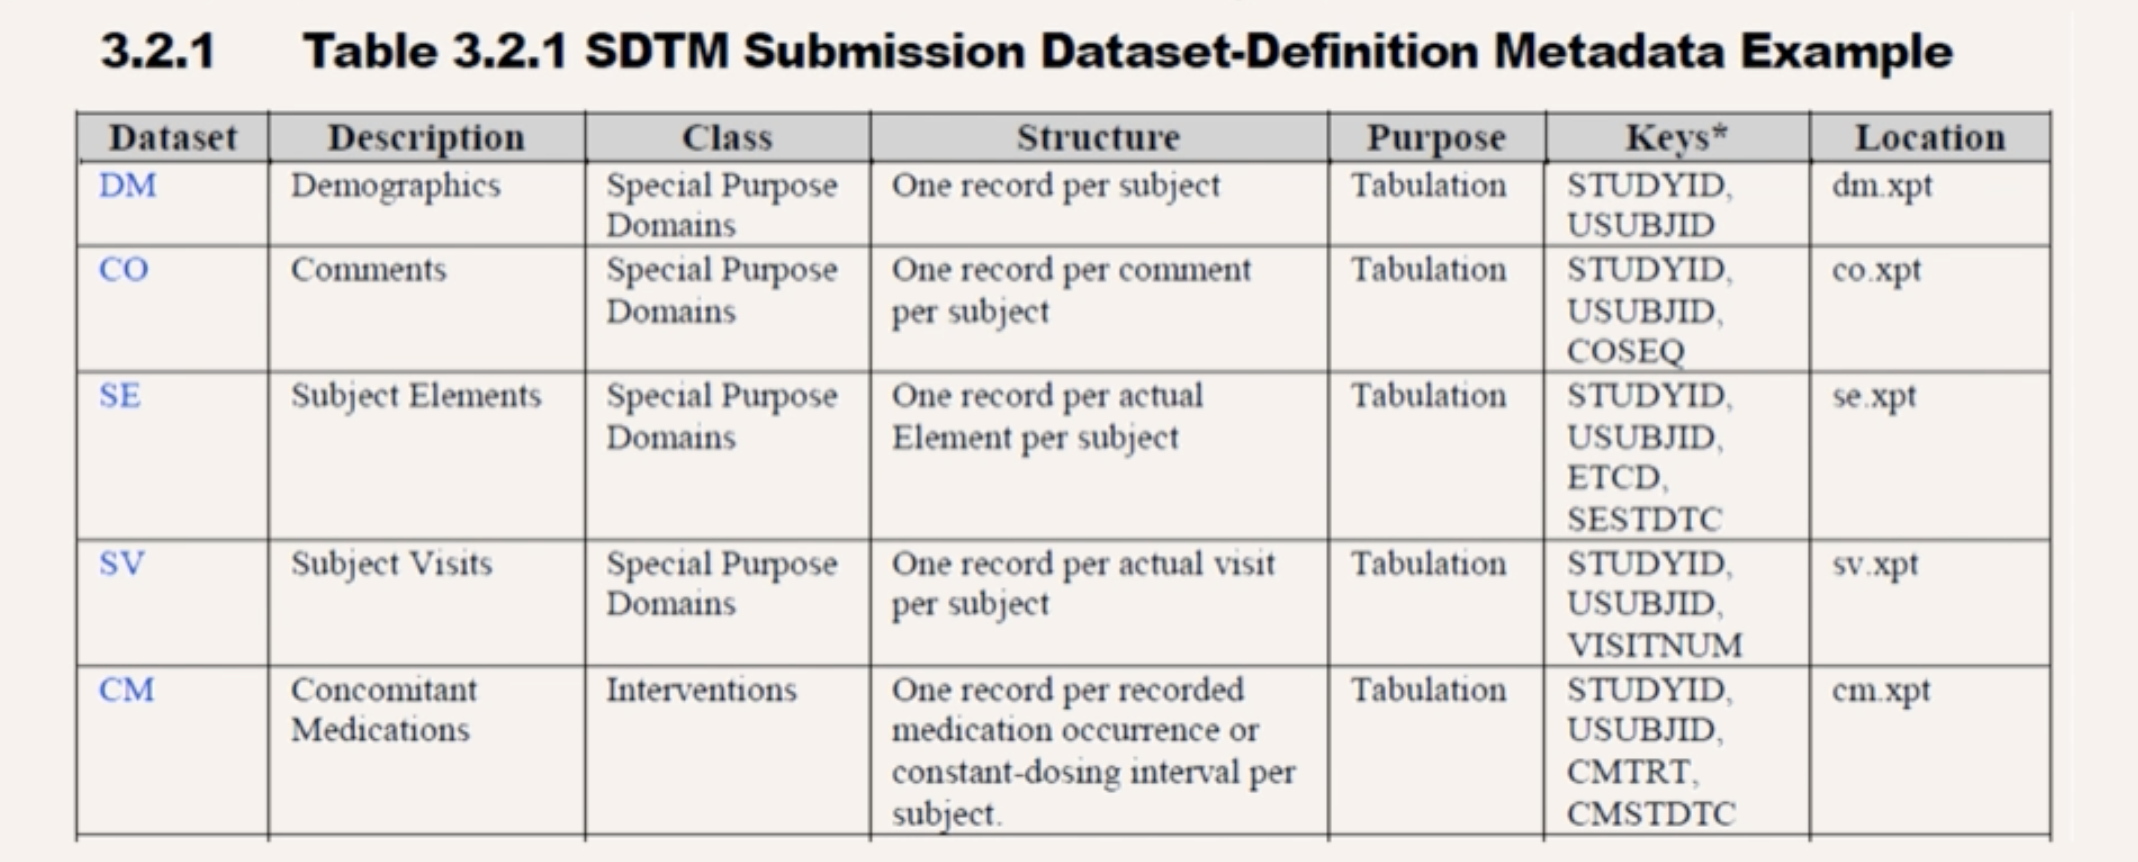
\includegraphics{/post/2021-10-10-biostatistical-note_files/WechatIMG685.png}

Deeper into DM detail:

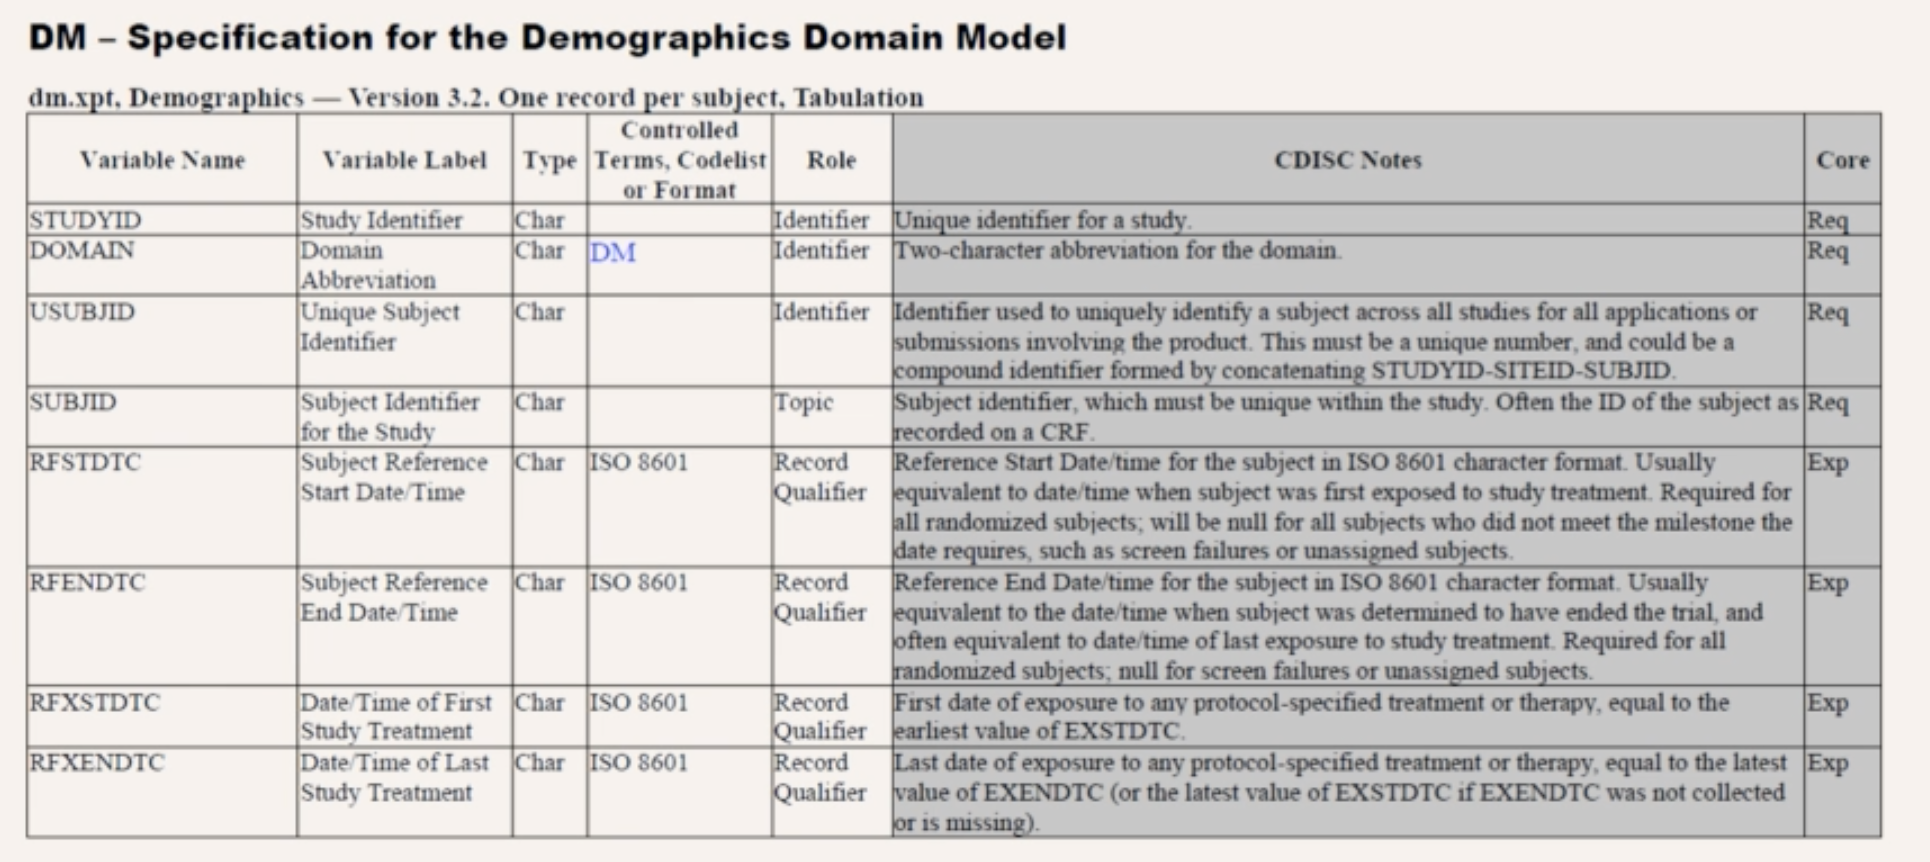
\includegraphics{/post/2021-10-10-biostatistical-note_files/WechatIMG686.png}

Definition of all standard domain models:
\url{https://en.wikipedia.org/wiki/SDTM}

\hypertarget{clinical-study-documents}{%
\paragraph{Clinical Study Documents}\label{clinical-study-documents}}

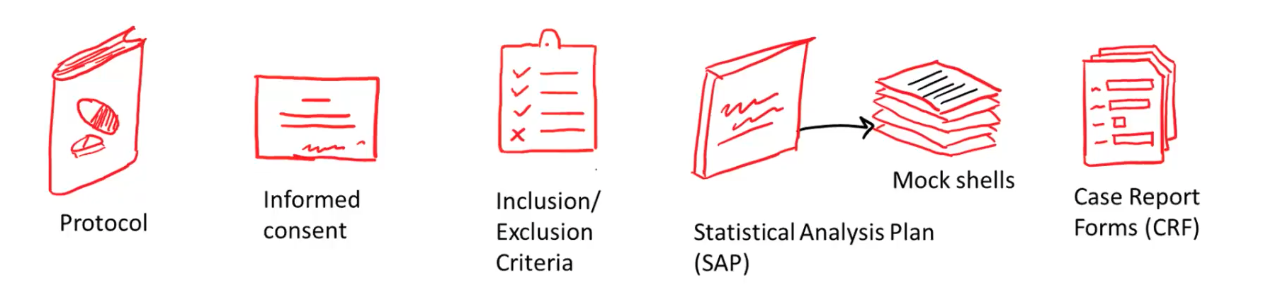
\includegraphics{/post/2021-10-10-biostatistical-note_files/22.jpg}

\begin{itemize}
\item
  \textbf{Protocol} A protocol is a strategy plan on which all clinical
  trials are based. Specific sections are listed on
  \url{https://irb.research.chop.edu/writing-protocol}. The sponsoring
  organization must approve the protocol and Institutional Review Board
  (IRB) at each study site reviews the protocol to ensure that
  participants are treated humanely and ethically. The IRB also
  discusses such issues as whether the likely benefit of the treatment
  is worth its risk.
\item
  \textbf{Informed Consent} All patients should sign the informed
  consent before they join the trails. The information in it includes
  details about experimental treatments, tests that must be given the
  possible risks and benefits of the tests, as well as any standard
  treatments available for their condition.
\item
  \textbf{Inclusion/Exclusion Criteria} Inclusion/Exclusion Criteria are
  the list of factors that allow/disallow someone from participating in
  the clinical trial.
\item
  \textbf{Statistical Analysis Plan (SAP)} The SAP is intended to be a
  comprehensive document that contains a detailed and technical
  description of the principal features of the analysis outlined in the
  protocol. It also includes detailed procedures for executing the
  statistical analysis of the primary and secondary variables and other
  data. As compared to the protocol, the SAP should contain an in-depth
  description of the statistical methods to be used and a definition of
  the statistical output which will be included in the clinical study
  report.
\item
  \textbf{Mock Shells} Mock shells is like the relational schema in SQL.
  It gives code programmer the general view of all datasets.
\item
  \textbf{Case Report Forms (CRF)} CRF is a printed, optical, or
  electronic document designed to record all protocol-required
  information on each subject in a clinical research study.
\end{itemize}

\hypertarget{abbreviation}{%
\subsubsection{\texorpdfstring{\textbf{Abbreviation}}{Abbreviation}}\label{abbreviation}}

A1C(HbA1C): Average Blood Glucose AE: Adverse Events ADE: Adverse Device
Effect BG: Blood Glucose CEC: Clinical Events Committee CGM: Continuous
Glucose Monitoring CR: Carb Ratio CRF: Case Report Forms CRS: Clinical
Research Specialist CIP: Clinical Investigation Plan CL: Closed Loop
CSM: Clinical Study Manager CSR: Clinical Study Report DD: Device
Deficiency DM: Data Manager DMC: Data Monitoring Committee DMP: Data
Management Plan DIA: Duration of Insulin Action DKA: Diabetic
Ketoacidosis EDC: Electronic Data Capture EOS: End of Study FDA: Food
and Drug Administration HCL: Hybrid Closed Loop IAC: Insulin Active
Curve IB: Investigator's Brochure ICF: Informed Consent Form IOB:
Insulin on Board ISF: Insulin Sensitivity Factor RAD: Regulatory Affairs
Domain SAP: Statistical Analysis Plan SAE: Serious Adverse Events SADE:
Serious Adverse Device Effect SG: Sensor Glucose SMBG: Self-Monitoring
of Blood Glucose SME: Subject Matter Expert TAR: Time Above Range TBR:
Time Below Range TDD: Total Daily Dose TIR: Time in Target Range TMF:
Trial Master File UADE: Unanticipated Adverse Device Effect UAT: User
Acceptance Testing USADE: Unanticipated Serious Adverse Device Effect

\hypertarget{knowledge-about-diabetes}{%
\subsubsection{\texorpdfstring{\textbf{Knowledge about
Diabetes}}{Knowledge about Diabetes}}\label{knowledge-about-diabetes}}

\textbf{Insulin} Insulin is a hormone made by the pancreas. Insulin
lowers blood glucose levels by allowing glucose to move out of the blood
and into your body's cells. The pancreas releases insulin 24 hours a
day. The insulin is released in two ways: A small amount (basal level)
of insulin is released in between meals and while you sleep. A larger
amount (a bolus) of insulin is released after eating. When you have
diabetes, you may not make any insulin or not make enough insulin. So
you rely on injectable insulin to lower your glucose levels.

\textbf{Glucagon} You can think of glucagon as the opposite of insulin,
because glucagon raises glucose levels. When a healthy pancreas senses
that glucose levels are dropping too low, it releases glucagon. Glucagon
tells the liver to release some off the glucose it stored into the blood
stream. As thee glucose enters the bloodstream, blood glucose levels
start to rise.

\textbf{Bolus vs Basal Insulin:} To manage diabetes, people may need
insulin and other medication to help control body sugar levels. The two
main ways to take insulin are bolus and basal. \texttt{Bolus\ insulin}
is the quick-acting delivery that you often take before mealtimes while
\texttt{basal\ insulin} is longer-acting and helps keep your glucose
levels steady day and night.

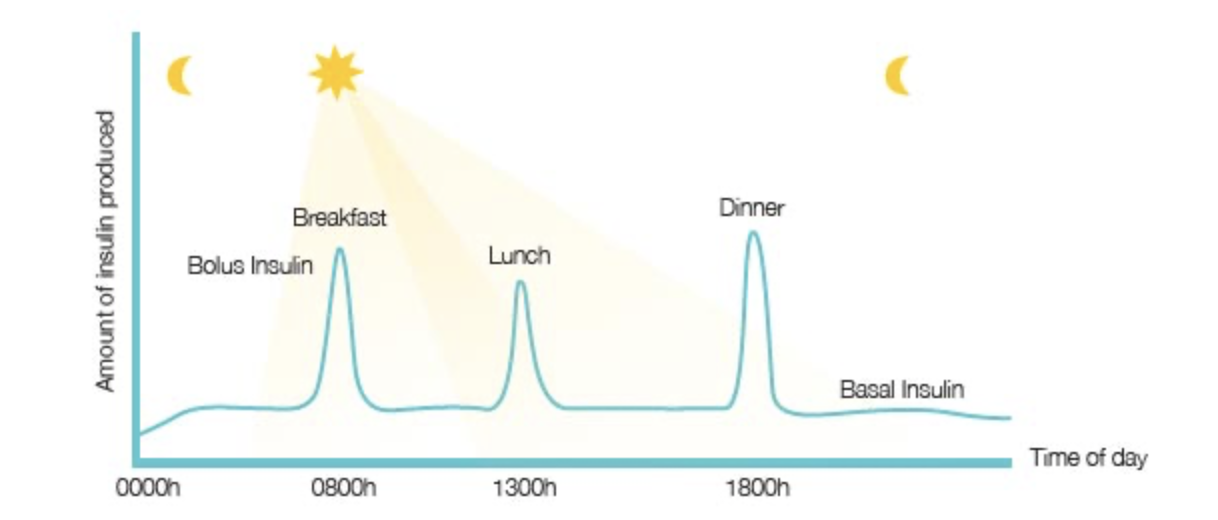
\includegraphics{/post/2021-10-10-biostatistical-note_files/WechatIMG669.png}

\textbf{Sensor Glucose vs Blood Glucose} Your sensor glucose (SG)
readings are taken from your interstitial fluid{[}组织液{]}, and not
from your blood (fingersticks).

\textbf{Type 1 and Type 2 Diabetes}

Type 1

Type 2

What is happening?

Your body attacks the cells in your pancreas which means it cannot make
any insulin.

Your body is unable to make enough insulin or the insulin you do make
doesn't work properly.

Risk factors

We don't currently know what causes type 1 diabetes.

We know some things can put you at risk of having type 2 like weight and
ethnicity.

Symptoms

The symptoms for type 1 appear more quickly.

Type 2 symptoms can be easier to miss because they appear more slowly.

Management

Type 1 is managed by taking insulin to control your blood sugar.

You can manage type 2 diabetes in more ways than type 1. These include
through medication, exercise and diet. People with type 2 can also be
prescribed insulin.

Cure and Prevention

Currently there is no cure for type 1 but research continues.

Type 2 cannot be cured but there is evidence to say in many cases it can
be prevented and put into remission.

\textbf{A1C} The A1C test-also known as the hemoglobin A1C or HbA1c
test-is a simple blood test that measures your average blood sugar
levels over the past 3 months. It's one of the commonly used tests to
diagnose prediabetes and diabetes, and is also the main test to help you
and your health care team manage your diabetes.

A normal A1C level is below 5.7\%, a level of 5.7\% to 6.4\% indicates
prediabetes, and a level of 6.5\% or more indicates diabetes. Within the
5.7\% to 6.4\% prediabetes range, the higher your A1C, the greater your
risk is for developing type 2 diabetes.

\textbf{The Glucose Area Under the Curve (AUC)} The glucose area under
the curve, which is an index of whole glucose excursion after glucose
loading, has been widely used for calculating the glycemic index and for
evaluating the efficacy of medications for postprandial hyperglycemia.

\textbf{Open Loop vs Closed Loop} Insulin therapy is one of the most
widely used methods for antidiabetic treatment. In contrast with
manually controlled open-loop insulin delivery devices, closed-loop
devices are continuously and automatically operated to mimic the natural
insulin production process of the pancreas.

\textbf{Carb Ratio} Your insulin-to-carb ratio (also just called a
``carb ratio'' or ``carb factor'') indicates how many grams of
carbohydrate one unit of rapid-acting insulin covers to ensure that your
blood glucose stay in your desired range. E.g. \emph{``If my carb ratio
is 1:10 and I'm eating 30 grams of carbs, I'll need 3 units of
rapid-acting insulin to cover the meal''}

\textbf{Types of Insulin} Terms to know:

\begin{itemize}
\tightlist
\item
  Onset - How quickly insulin lowers your blood sugar.
\item
  Peak Time - When insulin is at maximum strength.
\item
  Duration - How long insulin works to lower your blood sugar.
\end{itemize}

Insulin Type

Onset

Peak Time

Duration

Method

Rapid acting

15 minutes

1 hour

2 to 4 hours

Usually taken right before a meal. Often used with longer-acting insulin

Rapid-acting inhaled

10 to 15 minutes

30 minutes

3 hours

Usually taken right before a meal. Often used with injectable
long-acting insulin

Regular/short acting

30 minutes

2 to 3 hours

3 to 6 hours

Usually taken 30 to 60 minutes before a meal

Intermediate acting

2 to 4 hours

4 to 12 hours

12 to 18 hours

Covers insulin needs for half a day or overnight. Often used with rapid-
or short-acting insulin

Long acting

2 hours

Does not peak

Up to 24 hours

Covers insulin needs for about a full day. Often used, when needed, with
rapid- or short-acting insulin

Ultra-long

6 hours

Does not peak

36 hours or longer

Provides steady insulin for long periods

Premixed

5 to 60 minutes

Peak vary

10 to 16 hours

Combines intermediate- and short- acting insulin. Usually taken 10 to 30
minutes before breakfast and dinner

\textbf{Insulin Sensitivity Factor (ISF)} Insulin sensitivity factor or
``correction factor'' is how much one unit of insulin is expected to
lower blood sugar. For example, if 1 unit of insulin will drop your
blood sugar by 25 mg/dl, then your insulin sensitivity factor is 1:25.
In the example above, the pump would recommend 3 units of insulin to
bring blood glucose from 175 mg/dl down to 100 mg/dl. Different ISFs can
be pre-programmed for different times of the day -- e.g., many people
are more insulin resistant in the morning, which requires a stronger
correction factor.

\textbf{Duration of Insulin Action (DIA)} Duration of insulin action (or
active insulin time) is how long a bolus of insulin takes to finish
lowering blood glucose. The DIA time starts when a bolus is given and
ends when the bolus is no longer lowering blood glucose levels. An
accurate DIA will minimize insulin stacking and low blood sugar
(hypoglycemia), which can happen when boluses are given too close
together.

\textbf{Insulin on Board (IOB)} Insulin on board is how much insulin is
still active inside the body from the previous bolus dose. It is
calculated based on your DIA, though the exact calculation varies
depending on the pump. Roughly speaking, for a DIA of three hours, a
three-unit bolus dose taken at 12pm would have about one unit of IOB
remaining two hours later, at 2pm. IOB is important to take into
account, as it can help avoid insulin stacking. This is also helpful at
bedtime when determining whether or not you need more insulin to cover a
high reading.

\hypertarget{design-of-experiment}{%
\subsubsection{\texorpdfstring{\textbf{Design of
Experiment}}{Design of Experiment}}\label{design-of-experiment}}

\textbf{Multi-center} A multicenter research trail is a clinical trail
conducted at more than one medical center or clinic. Most large clinical
trails, particularly Phase III trails, are conducted at several clinical
research centers

\textbf{Single-arm Trial} The simplest trial design is a single-arm
trial. In this design, a sample of individuals with the targeted medical
condition is given the experimental therapy and then followed over time
to observe their response.

\textbf{Randomized Controlled Trial (RCT)} RCT is a study in which
people are allocated at random (by chance alone) to receive one of
several clinical interventions. One of these interventions is the
standard of comparison or control. The control may be a standard
practice, a placebo (``sugar pill''), or no intervention at all. RCTs
seek to measure and compare the outcomes after the participants receive
the interventions.

\textbf{Parallel Group Study} When every participant receives one and
only one treatment in a random manner, this kind of complete randomized
design is called a parallel group design. The most important element of
this design is randomization which means participants are randomly
placed into a group to lower the risk of statistical bias or other kinds
of erroneous results.

Generally, researchers use either one of the two types of parallel group
designs in a comparative clinical trial, that is, parallel group (or
group comparison) designs or matched-pair parallel designs (Figure
below). Based on certain characteristics, participants are first paired
in matched-pair parallel design. Within one pair, each member will be
assigned to different study subgroups randomly, which makes it possible
to compare similar participants undergoing diverse procedures between
each other. A treatment group vs.~a control group is the simplest
two-group comparison parallel-group design. In each treatment group
there are usually the nearly same amount of participants that's not
always the case.

A parallel group design is very different from a crossover design in
which one group of participants receives treatment A first followed by B
then while the other group does the opposite. However, there is also a
significant issue in a parallel trial. Researchers must take into
consideration the intra subject variability, the variability within the
same participants in responses to treatment.

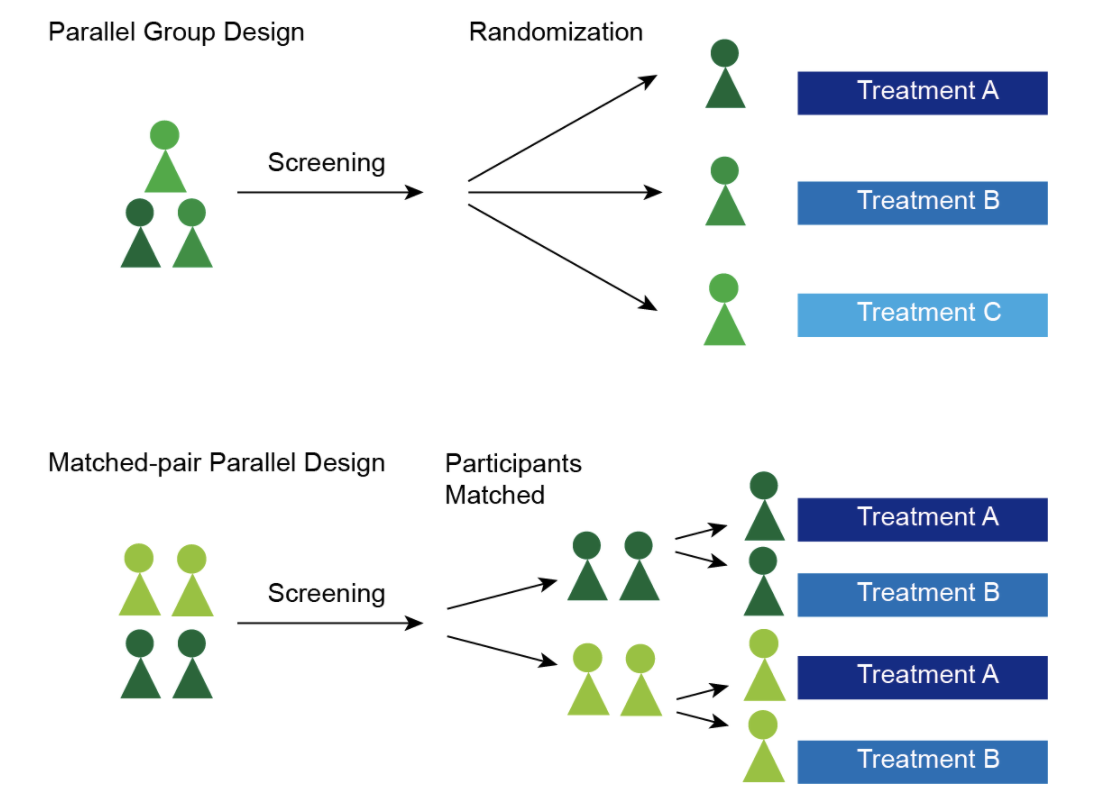
\includegraphics{/post/2021-10-10-biostatistical-note_files/WechatIMG667.png}

\textbf{Cross-over Study} The AB/BA model is the simplest type of
crossover trial. At first, participants of one group will receive
medication A and after a wash-out period, participants of the same group
will receive medication B. The same applies to the second study group,
but the other way around. Extensions to this form include the
ABC/CBA/BCA regimens.

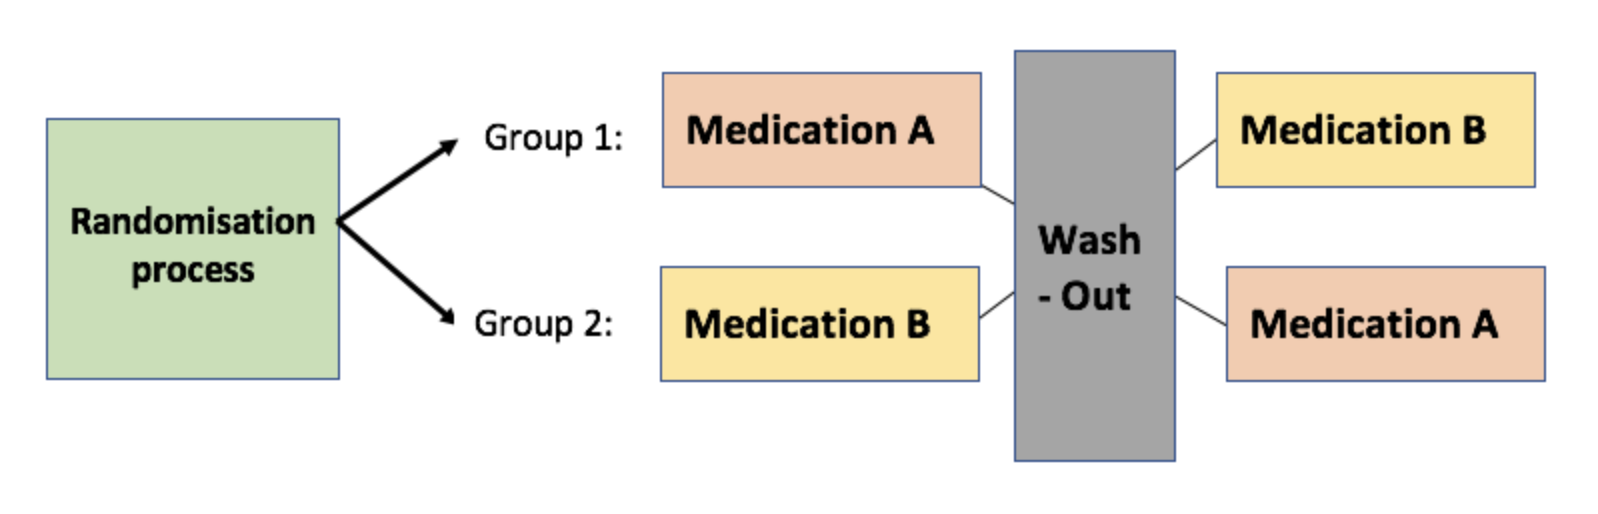
\includegraphics{/post/2021-10-10-biostatistical-note_files/WechatIMG666.png}

\emph{Advantages} By using a crossover trial in order to compare several
interventions, a researcher can minimize the risk of confounding because
all interventions are measured on the same participants. One can say
that study participants serve as their own control. This leads to
another advantage which is less study participants are required compared
to a standard parallel randomized controlled trial (RCT). Reduction of
sample size is consistent with the principle in medical research to use
resources wisely. Furthermore, blinding of study participants can be
maintained and statistical tests assuming randomization can be used.

\emph{Limitations} This design sounds very appealing, however there are
various limitations that need to be considered:

\begin{enumerate}
\def\labelenumi{\arabic{enumi}.}
\item
  Crossover trials can only be conducted when the disease persists for a
  longer period of time, hence, crossover trials are mostly used in
  studying chronic diseases. There are some short-term illnesses or
  acute conditions that might be cured once they are treated and there
  are treatments that will have a permanent effect (i.e.~surgery) on the
  patient. It is usually not possible to perform crossover trials in
  such cases.
\item
  There is a great risk for aliasing. This term describes the risk that
  there might be a carry-over from the effect of the previous
  intervention on to the effect of the next intervention thereby
  altering results. Therefore, the treatment effect might not only be
  due to the treatment itself, but also due to interactions between
  treatment and study-period/sequence. Statistical tests have been
  suggested in order to test the carry-over risk, but a great chance of
  a type-II error (falsely accepting the null hypothesis, here: falsely
  accepting the hypothesis that there is no interaction between
  treatment and study-period or study-group) persists.
\item
  It is difficult to estimate the time required in order for the
  intervention to be fully washed-out. While it might be relatively
  simple to estimate the wash-out period when the intervention is given
  as a drug looking at the half-life of the studied medications, things
  become a lot trickier when the interventions include psychological
  therapies, for example.
\item
  In contrast to parallel designs, crossover trials consist of two study
  periods. This means that they usually take up more time, and
  statistical analysis can be more complicated if participants do not
  complete all stages of the trial.
\end{enumerate}

In conclusion, crossover trials are a good study design that can be used
to efficiently compare interventions on as few participants as possible
when studying chronic diseases. However, many requirements (low risk of
carry-over, wash-out period etc.) must be met and therefore it is not
used as often as a parallel RCTs.

\textbf{Prospective vs Retrospective Study} Both prospective and
retrospective study are a kind of cohort study. In prospective study,
researchers take all subjects into account before they start developing
noteworthy outcomes. In retrospective study, researchers focus on two
groups of subjects: One with disease, the other similar one but without
disease. E.g.

\begin{itemize}
\tightlist
\item
  Prospective Study(前瞻性研究):
  对100名有肺癌高危因素的人进行为期10年的跟踪调查,看看他们是否患上了肺癌。
\item
  Retrospective Study(回顾性研究):
  对50名抽烟患有肺癌的人和50名抽烟但不患肺癌的人进行调查,对比他们之前的各种生活习惯等。
\end{itemize}

\hypertarget{statistical-knowledge}{%
\subsubsection{\texorpdfstring{\textbf{Statistical
Knowledge}}{Statistical Knowledge}}\label{statistical-knowledge}}

\textbf{What is Power} Power is the probability of rejecting the null
hypothesis when in fact it is false. Power is the probability of making
a correct decision (to reject the null hypothesis) when the null
hypothesis is false.

\textbf{ITT Principle} The intention-to-treat (ITT) principle is a
cornerstone in the interpretation of randomized clinical trails
conducted with the goal of influencing the selection of medical therapy
for well-defined groups of patients. The ITT principle defines both the
study population included in the primary effect analysis and how the
outcomes are analyzed.

Under ITT, study participants are analyzed as members of the treatment
group to which they were randomized regardless of their adherence to, or
whether they received, the intended treatment. For example, in a trail
in which patients are randomized to receive either treatment A or
treatment B, a patient may be randomized to receive treatment A but
erroneously receive treatment B, or never receive any treatment, or not
adhere to treatment A. In all of these situations, the patient whould be
included in group A when comparing treatment outcomes using an ITT
analysis.

\textbf{\emph{References}}

\emph{1. Udemy: The Simplest Guide to Clinical Trails Data Analysis with
SAS:
\url{https://www.udemy.com/course/the-simplest-guide-to-clinical-sas-programming/}}
\emph{2.
\url{https://www.cdc.gov/diabetes/managing/managing-blood-sugar/a1c.html}}
\emph{3.
\url{https://www.diabetes.org.uk/diabetes-the-basics/differences-between-type-1-and-type-2-diabetes}}
\emph{4. \url{https://aip.scitation.org/doi/abs/10.1063/5.0049209}}
\emph{5. \url{https://diabetesstrong.com/insulin-to-carb-ratios/}}
\emph{6.
\url{https://www.cdc.gov/diabetes/basics/type-1-types-of-insulin.html}}
\emph{7.
\url{https://jamanetwork.com/journals/jama/article-abstract/1884555}}
\emph{8.
\url{https://s4be.cochrane.org/blog/2020/09/07/crossover-trials-what-are-they-and-what-are-their-advantages-and-limitations/}}
\emph{9.
\url{https://www.medicinenet.com/randomized_controlled_trial/definition.htm}}
\emph{10. \url{https://www.cd-biosciences.com/parallel-group-design/}}
\emph{11.
\url{https://www.healthxchange.sg/diabetes/essential-guide-diabetes/what-is-type-1-diabetes}}
\emph{12.
\url{https://diatribe.org/understanding-insulin-pump-settings}}
\emph{13. Udemy: Hack into SAS Clinical Trials Programming
Certification:
\url{https://www.udemy.com/course/hack-into-sas-clinical-trials-programming-certification/}}

\end{document}
